\chapter{Familias de gramática de atributos}
\label{chap:clas_ag}
\minitoc

Las familias de GA pueden ser clasificadas, principalmente, teniendo en cuenta dos aspectos: según la \textbf{estrategia de evaluación} y según las \textbf{dependencias entre los atributos}. 

Las primeras, se basan en procedimientos de evaluación previamente definidos, en donde la idea es hacer varios recorridos del árbol atribuido e ir evaluando los atributos que sean posibles en cada uno de ellos. Luego de varios recorridos todos los atributos deberían estar evaluados (por supuesto si el grafo de dependencias es acíclico). Esta estrategia requiere que se tenga información sobre las dependencias entre los atributos durante la evaluación. Con respecto a las segundas, las GA presentan dependencias entre sus atributos que tienen ciertas características que permiten determinar estáticamente\footnote{Analizando las reglas de atribución de las producciones.} un orden total de sus instancias de atributos para cada producción que sea consistente con sus dependencias. 

Cada una de las familias de gramática de atributos tiene su propio poder expresivo, como así también, sus restricciones en el método de evaluación. La relación entre estos dos aspectos esta dado por el siguiente razonamiento: \textit{mientras más restricciones en el método de evaluación, menos poder expresivo}.

En el desarrollo de este capítulo se presentaran algunas de las familias de GA desde el punto de vista de las dependencias entre sus atributos\footnote{La familia de gramáticas analizadas desde el punto de vista de la estrategia de evaluación no serán abordadas, debido a que escapan al propósito del trabajo realizado. Las mismas pueden ser consultadas en \cite{tesismarcelo}.}, a solo efecto de abordar una comparación final y aportar una marco teórico adecuado para el análisis de gramáticas de atributos multi-plans (MAG). Las MAG, son analizadas en el capítulo siguiente y además son en las que se basa el desarrollo de \maggen. 

En el presente capítulo, no se profundizará demasiado en los métodos de evaluación de cada familia. Este tema es detallado por Marcelo Arroyo en \cite{tesismarcelo}, Wuu Yang en \cite{wuu-yang2} y U. Kastens en \cite{kastens}.

\section{Gramáticas de Atributos bien definidas (WDAG)}
\label{sec:well-defined}

Las \textit{gramática de atributos bien definida},(o \textit{well-defined}) es una familia basada en la estrategia de evaluación. En esta sección se presentará dicha familia y al final del capítulo se analizará su relación con las demás. 

\begin{definition} \label{def:gacompleta}Una gramática de atributos es completa si cumple con las siguientes propiedades:
\begin{enumerate}
\item Para toda producción $p \in P$, de la forma $p:X \rightarrow \chi$, todos los atributos sintetizados de $X$ se definen en $p$.
\item Para toda producción $p \in P$, de la forma $p:Y \rightarrow \mu X \nu$, todos los atributos heredados de $X$ se definen en $p$.
\end{enumerate}
\end{definition}

\begin{definition} 
Una gramática de atributos es \textbf{bien definida (WDAG)\footnote{En inglés Well Defined, de allí la abreviatura WD.}} si es completa y no se detectan planes con dependencias circulares.
\end{definition}

\section{Gramática de Atributos ordenadas (OAG)}
\label{sec:def-oag}
En cada gramática de esa clase, los atributos de un símbolo $X \in \Sigma$ pueden ser evaluados en un orden (total) determinado, es decir que es posible determinar un orden de evaluación independientemente de su contexto.
Esta información se puede utilizar para producir evaluadores para esta familia que sean muy eficientes, tanto en tiempo como en espacio y el algoritmo de verificación de circularidad tiene tiempo polinomial.

\begin{definition} Dada una GA, una familia de órdenes totales $O=\{O(X)\}$, donde cada $ O(X) $ es un orden total sobre los atributos del símbolo $ X \in \Sigma $, es consistente con el grafo de dependencias de la producción $p: X_0 \rightarrow X_1 X_2 \ldots X_{np}$, si el grafo de dependencias aumentado con dichos órdenes es no circular:

$$ DP_{ord}(p) \equiv DP(p) \cup \{ (X.a, X.b) \in O(X) \mid \textrm{X ocurre en p} \} $$
\end{definition}

\begin{definition} Una gramática de atributos es (ordenada) (OAG) si para cada producción existe un orden total, es decir que cada grafo $ DP_{ord}(p) $ no es circular.
\end{definition}

En 1996, Wuu Yang\cite{wuu-yang4} caracterizó una extensión a las OAG que permite que el algoritmo de decisión de pertenencia a esta nueva familia sea de tiempo polinomial. A ésta extensión se la conoce como \textbf{Extended OAG o EOAG}.

El algoritmo propuesto, se basa en la introducción de un paso adicional, previo a la construcción del particionado, que consiste en el armado de conjuntos de dependencias aumentadas de los símbolos y redefine el particionado para que se tengan en cuenta estas dependencias.
Marcelo Arroyo en \cite{tesismarcelo} presenta un análisis detallado sobre esta familia y  los algoritmos que propuso Wuu Yang.

\section{Gramática de Atributos absolutamente no circulares (ANCAG)}

Esta familia de gramáticas de atributos, denominada también \emph{fuertemente no circulares}) no comprende las GAs cuyas dependencias entre sus atributos es tal que cada atributo sintetizado del símbolo \textit{head} de cada producción,depende (directa o indirectamente) de un conjunto de sus atributos heredados.

Es posible definir formalmente que una GA es \emph{ANCAG} si se extiende el grafo de dependencias de cada producción $p: X_0 \rightarrow X_1 X_2 \ldots X_{np}$:

$$ IDP_{ANCAG} = \bigcup_{p \in P} IDP_{ANCAG}(p) $$

$$ IDP_{ANCAG}(p) = DP(p) \cup \{ (X.a,X.b) \mid
                             \exists q: X \rightarrow \alpha \: \in \: P $$
                $$ \land \: (X.a,X.b) \in IDP_{ANCAG}(q) \} $$

\begin{definition} Una gramática de atributos es ANCAG si ningún grafo $ IDP_{ANCAG}(p) $, para toda producción $p$, es circular.
\end{definition}

Notar que la relación $IDP-ANCAG(p)$ es pesimista ya que podría contener dependencias que nunca se podrían dar simultáneamente en un árbol sintáctico. Es decir, un grafo $IDP-ANCAG(p)$ contiene todas las dependencias transitivas entre los atributos que ocurren en $p$ para la unión de todos los posibles contextos inferiores. Este enfoque permite puntualizar ciclos en las dependencias que tienen poco sentido a efectos prácticos.

En el capítulo siguiente se retomará esta familia, con la definición \ref{def:ancag} y los teoremas \ref{th:ancag1} y \ref{th:ancag2} para cubrir su relación con la familia MAG.

\section{Gramáticas de Atributos no circulares (NC)}
\label{sec:gramNC}
En 1999 Wuu Yang\cite{wuu-yang2} propone una nueva clasificación de \emph{Gramáticas de atributos no circulares basadas en información de contextos inferiores (lookahead behavior)}. Esta jerarquía fue denominada por Wuu Yang como  \emph{\textbf{NC}}.

La idea básica en la jerarquía \emph{NC} es tratar de computar grafos de dependencias inducidos para cada producción y cada símbolo no terminal, que sean aproximaciones más reales (refinamientos) a los grafos utilizados en la caracterización de otras clases como las descriptas anteriormente. 

Es posible encontrar aproximaciones más exactas si se tienen en cuenta los posibles contextos inferiores de una instancia de aplicación de una producción. Esto a diferencia de las ANCAG que construyen grafos de dependencias sin tener en cuenta los posibles contextos y reales y penalizan en posibles dependencias cíclicas inútiles prácticamente. 

La jerarquía \emph{NC} se clasifica en clases según el \textit{lookahead behavior}. Este mide el nivel de transitividad en la observación de los posibles contextos inferiores de una producción.

Ahora se analizarán algunas de las clases en la jerarquía \emph{NC}:

\begin{description}
\item [NC(0)] Esta clase (sin $lookahead$) se corresponde con la familia ANCAG, debido que no observa contexto inferiores. 
\item [NC(1)] Las gramáticas $NC(1)$ mantienen un $lookahead$ de 1 y un resultado importante es que la familia $NC(1)$ contiene a las ANCAG. Wuu Yang en \cite{wuu-yang1} presenta la familia de las MAG y las asocia con esta subfamilia dentro de la jerarquía $NC(1)$. Es por ello que en el capítulo siguiente es tratada en detalles esta familia de gramáticas.
\item[NC(k)] Esta clase tiene en cuenta un $k>1$, es decir un $lookahead$ de $k$. La clase $NC(k)$ consiste de aquellas GA's para las cuales existe un conjunto de planes de evaluación para cada producción, que quedan determinados analizando $k$ niveles de producciones descendientes. Es decir $k$ niveles de observación en los posibles contextos inferiores.
\item[NC($\infty$)] Existen gramáticas de atributos que no pertenecen a la familia $NC(k)$ para ningún $k$. Esto sucede cuando la gramática tiene producciones que son mutuamente recursivas. Un árbol sintáctico podría contener derivaciones de la forma $X \rightarrow Y \rightarrow X$ para cualquier número de repeticiones y si existiera un ciclo en las dependencias no podría determinarse estáticamente para ningún número finito de descendientes $k$.

Un evaluador para las GA $NC(\infty)$ necesita tener en cuenta un número \emph{potencialmente (no realmente)} infinito de descendientes. En términos de un árbol sintáctico, lo anterior significa que el evaluador necesitará ``mirar'' hasta las hojas para seleccionar un plan para una instancia de una producción.

\begin{theorem} La familia $NC(\infty)$ se corresponde con la familia de gramáticas de atributos bien definidas (WDAGs).
\end{theorem}
\end{description}

Un resultado importante presentado por Wuu Yang en \cite{wuu-yang2} es el siguiente:
\begin{theorem}
Dado un $k$ finito, $NC(k)$ es una subclase propia de $NC(k+1)$ y existe un procedimiento de decisión para $NC(k)$.
\end{theorem}


\section{Relación entre familias}
\label{sec:relfamag}
A continuación, se analiza la relación entre familias de GA que fueron presentadas en este capítulo. El enfoque del análisis esta dado por el poder expresivo de cada familia (Ver tabla \ref{jer-GA} y la figura \ref{jer-GA2}).

\begin{table}[!ht]\centering
\begin{tabular}{ll}
\textbf{AG}         & Gramáticas de atributos \\
\textbf{WDAG o NC($\infty$)}       & Gramáticas de atributos bien definidas\\
\textbf{NC(k)}       & Gramáticas de atributos no circulares con $k > 1$\\
\textbf{MAG o NC(1)}       & Gramáticas de atributos Multi-plans\\
\textbf{ANCAG o NC(0)}      & GA absolutamente no circulares \\
\textbf{EOAG}       & GA Ordenadas Extendidas \\
\textbf{OAG}        & GA Ordenadas \\
% \hline
% \textbf{m-APAG}     & GA evaluables en \emph{m} pasadas alternantes \\
% \textbf{n-PAG}      & GA evaluables en \emph{n} pasadas \\
% \textbf{L-AG}       & GA l-atribuidas \\
% \textbf{S-AG}       & GA s-atribuidas \\
\end{tabular}
\caption{Jerarquía de GA}
\label{jer-GA}
\end{table}

\begin{figure}\centering
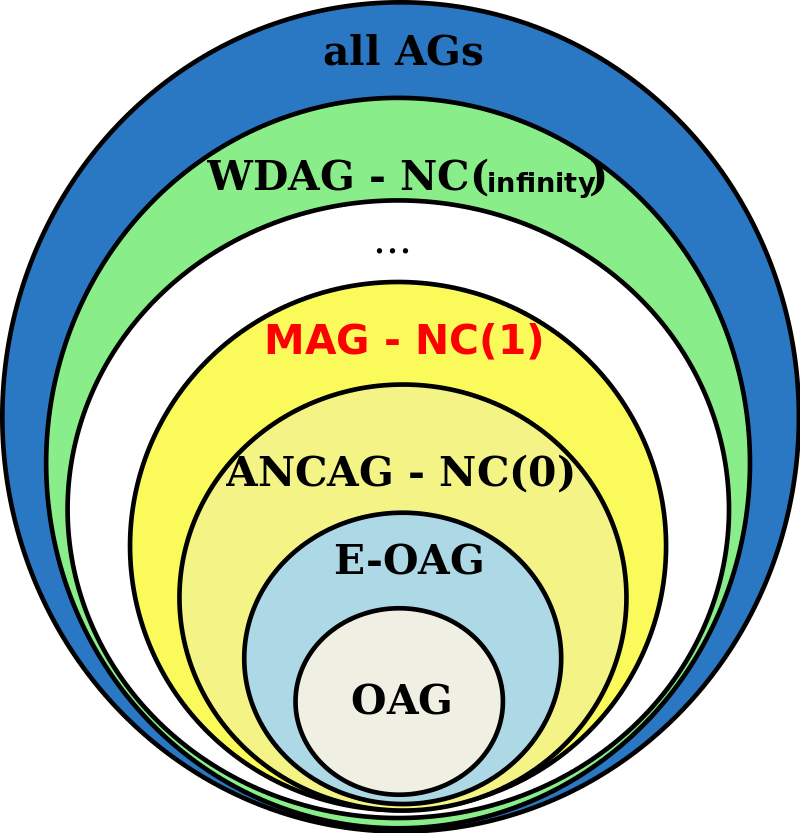
\includegraphics[width=250pt,height=260pt]{familias-ag.png}
\caption{\label{jer-GA2}Relación entre familias de gramáticas de atributos.} 
\end{figure}

En la relación mostrada arriba se incluye la familia MAG, la cual será analizada en el capítulo siguiente.
Detalles sobre demostraciones acordes a las inclusiones presentadas son tratadas ampliamente por Marcelo Arroyo en \cite{tesismarcelo}.